\documentclass[12pt]{arstexnica}
\usepackage[italian]{babel}
\usepackage[latin1]{inputenc}
\usepackage[T1]{fontenc}
\usepackage{graphicx, guit, multicol, overpic, lmodern, microtype,textcomp}

\geometry{margin=2cm,onecolumn}

\usepackage{hyperref}

\setlength{\parindent}{0pt}

\guitcolor[rgb]{0,0.6,0}
\colorlet{poster}{coloredelGuIT}


\begin{document}
\pagestyle{empty}

\begin{center}
  \begin{overpic}[width=.9\textwidth]{GuITTeX}
    \put(65, 25){%
      \fontfamily{pzc}\fontsize{70}{80}\selectfont
      \color{poster}2014}
    \put(-5, 57){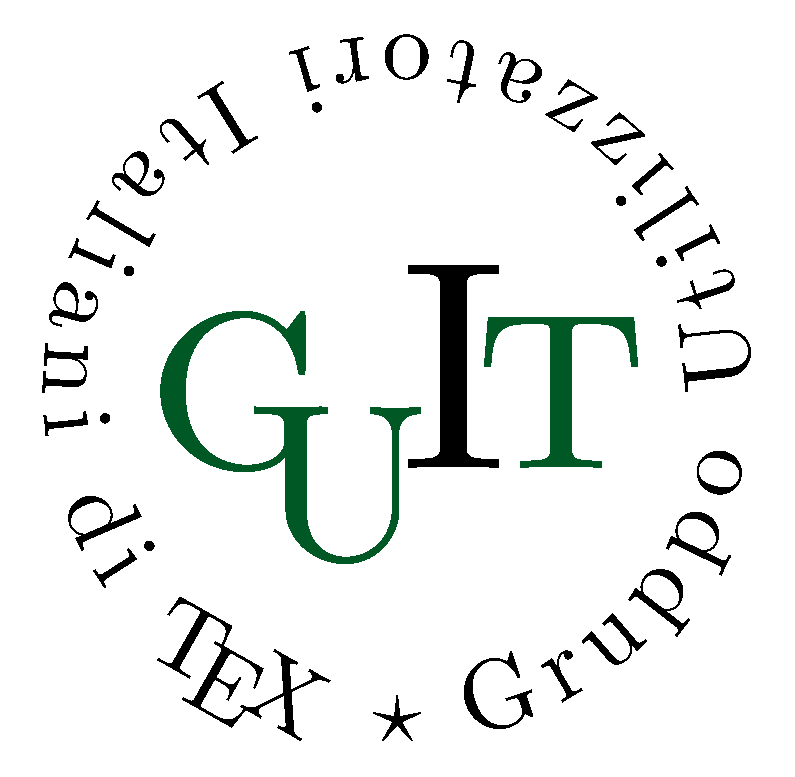
\includegraphics[width=.18\textwidth]{logotondoGuIT}}%
%    \put(65, 60){\includegraphics[width=.4\textwidth]{SSSA_col}}
  \end{overpic}

  \vspace{\stretch{1}}

  \Huge\bfseries\sffamily
  Undicesimo convegno nazionale su \TeX, \LaTeX\ e tipografia digitale

  \bigskip

  \LARGE\mdseries\color{poster}
  Verona, 18 ottobre 2014

  \bigskip

  \normalcolor
  Tema principale:\\``TeX come strumento per la scrittura accademica''
\end{center}

\begin{center}
\textbf{Call for Papers}
\end{center}

Sabato 18 ottobre a Verona si terr� l'undicesimo Convegno annuale su
\TeX, \LaTeX\ e tipografia digitale organizzato dal \GuITtext. Il 
Convegno sar� un momento di ritrovo e di confronto per la comunit�
\LaTeX\ italiana, tramite una serie di interventi atti sia a
contribuire all'arricchimento sia a supportarne lo sviluppo.

Maggiori informazioni sul Convegno e sulle modalit� di presentazione
degli interventi saranno disponibili all'indirizzo:

\begin{center}
\texttt{http://www.guitex.org/guitmeeting/2014/}
\end{center}

\vspace{\stretch{4}}



\end{document}
